\documentclass[11pt,a4paper]{report}
\usepackage{inputenc} 
\usepackage[english]{babel} 
\usepackage{graphicx}
\usepackage{a4wide}
\usepackage[dvipsnames]{xcolor}
\usepackage{tikz}
\usepackage{lipsum}
\usepackage{listings}
\usepackage{cleveref}
\usepackage{placeins}

%Remove trailing zero in section numbering
\renewcommand{\thesection}{\arabic{section}}

%\lstset{
%  basicstyle=\ttfamily,
%  keywordstyle=\textcolor{blue},
%  language=XML,
%  morekeywords={<ScalarVariable,Real}
%}

\renewcommand{\ttdefault}{pcr}

\lstdefinelanguage{XML}
{
  basicstyle=\ttfamily\footnotesize,
  morestring=[b]",
  moredelim=[s][\bfseries\color{Maroon}]{<}{\ },
  moredelim=[s][\bfseries\color{Maroon}]{</}{>},
  moredelim=[l][\bfseries\color{Maroon}]{/>},
  moredelim=[l][\bfseries\color{Maroon}]{>},
  morecomment=[s]{<?}{?>},
  morecomment=[s]{<!--}{-->},
  commentstyle=\color{DarkOliveGreen},
  stringstyle=\color{blue},
  identifierstyle=\color{red}
}

\begin{document}

\title{Wrapper for Functional Mock-up Interface in TLM-based Asynchronous Co-Simulation}
\author{Robert Braun}

\maketitle

\section{Introduction}
Functional Mock-up Interface (FMI) is a tool-independent standard for connecting simulation tools. 
One tool can export a model as a Functional Mockup Unit (FMU), a ZIP package with the file extension FMU. 
This file is in turn loaded by the master simulation tool, which can connect and simulate the model.
An FMU file contains a model description XML file called \texttt{modelDescription.xml}, binaries for different platforms and other optional content.
It is important that the FMU contains a binary file for the platform where the master simulation tool is executed.

There are two versions of the FMI standard: FMI for Co-Simulation and FMI for Model Exchange.
The main difference is that FMUs for Co-Simulation contain their own built-in solvers, and only exchange data at predefined communication points.
FMUs for Model Exchange require a solver in the master simulation tool.

Including FMUs in the TLM framework requires a wrapper.
\texttt{FMIWrapper} is a generic wrapper for connecting functional mockup units (FMUs) to the TLM framework.
It uses the FMI Library from Modelon to load an FMU, and the TLMPlugin for socket communication with the framework, see \cref{fig:overview}.

\begin{figure}[ht]
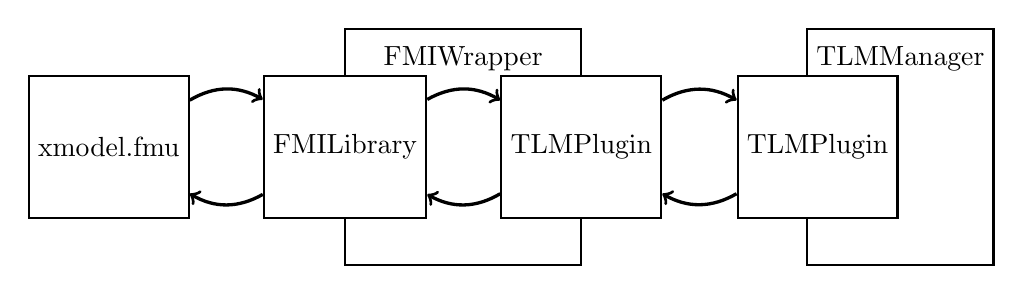
\begin{tikzpicture}
\def\dx{0.0495*\textwidth}

\node[rectangle,draw,thick, 
      minimum width=5*\dx, 
      minimum height=5*\dx, 
      text depth=5*\dx-20pt] () {FMIWrapper};

\node[rectangle, draw, thick, 
      minimum width=3*\dx, 
      minimum height=3*\dx, 
      xshift=2.5*\dx,
      fill=white] (tp1) {TLMPlugin};
      
\node[rectangle, draw, thick, 
      minimum width=3*\dx, 
      minimum height=3*\dx, 
      xshift=-2.5*\dx,
      fill=white] (fl) {FMILibrary};
      
\node[rectangle, draw, thick, 
      minimum width=3*\dx, 
      minimum height=3*\dx, 
      xshift=-7.5*\dx] (fmu) {xmodel.fmu};

\node[rectangle, draw, thick, 
      minimum width=3.5*\dx, 
      minimum height=5*\dx, 
      text depth=5*\dx-20pt,
      xshift=9.25*\dx,
      fill=white] () {TLMManager};

\node[rectangle, draw, thick, 
      minimum width=3*\dx, 
      minimum height=3*\dx, 
      xshift=7.5*\dx,
      fill=white] (tp2) {TLMPlugin};

\draw[thick,->,very thick] (fmu) edge[bend left] (fl);
\draw[thick,<-,very thick] (fmu) edge[bend right] (fl);
\draw[thick,->,very thick] (fl) edge[bend left] (tp1);
\draw[thick,<-,very thick] (fl) edge[bend right] (tp1);
\draw[thick,->,very thick] (tp1) edge[bend left] (tp2);
\draw[thick,<-,very thick] (tp1) edge[bend right] (tp2);
\end{tikzpicture}
\caption{Blabla...}
\label{fig:overview}
\end{figure}

Both FMI for co-simulation and FMI for model exchange are supported. 
Model exchange requires a solver in the wrapper executable.
For this reason, two solvers from the Sundials package are included.

\section{Setting up a simulation}
The FMI wrapper is started by the StartTLMFMIWrapper startup script.
This script generates the \texttt{tlm.config} fileand calls the FMIWrapper executable.
The executable takes the following arguments:\\

\noindent \verb|FMIWrapper <path> <fmufile> <solver> <debug>|\\

Example:\\

\noindent \verb|FMIWrapper C:\temp\folder mymodel.fmu solver=CVODE -d|\\

The last to arguments are optional.
Available solvers are \texttt{Euler}, \texttt{CVODE} and \texttt{IDA}.
These can currently only be changed by modifying the startup script, i.e. not from the graphical interface.

An FMU keep track of its variables by integer numbers called \texttt{value references}.
However, it does not provide any information about the mapping between its variables and the TLM interface.
Hence, this information must be provided by the user.
A configuration file called \texttt{fmi.config} is used for this purpose, see \cref{lst:fmiconfig}.

\begin{lstlisting}[basicstyle=\ttfamily,floatplacement=ht,caption="Blabla",label=lst:fmiconfig]
substeps,100
name,tlm1
position,6,7,8
orientation,136,139,142,137,140,143,138,141,144
speed,9,10,11
ang_speed,145,146,147
force,133,134,135,167,168,169
name,tlm2
position,...
\end{lstlisting}

As can be seen, data is stored in a comma-separated format.
The first line specifies the number of substeps used for FMI for Co-Simulation (see \cref{sec:fmi_cs}).
After this comes the port information.
Each port is specified by name, position, orientation, speed, angular speed and force, according to the TLM interfaces in the TLM framework.
The numbers after each keyword are the value references.
These can be obtained by analyzing the \texttt{modelDescription.xml} file.
\Cref{lst:modeldescription} shows an example.
The variable first torque component has the value reference 167.
Hence, this number should be inserted as number four on the "force" line in \texttt{fmi.config}.

\begin{lstlisting}[language=XML,floatplacement=ht,caption="Blabla",label=lst:modeldescription]
  <ScalarVariable
    name="fMITLMInterface3D1.t[1]"
    valueReference="167"
    variability="continuous"
    causality="local"
    >
    <Real/>
  </ScalarVariable>
\end{lstlisting}



\FloatBarrier
\section{FMI for Co-Simulation}
\label{sec:fmi_cs}
With FMI for Co-Simulation the solver is embedded within the FMU.
Variables can only be exchanged at predefined communication points.
Hence, it is not possible for the solver to obtain interpolated force variables during internal iteration steps.
Keeping the force constant during the entire communication interval may, however, have a negative effect on numerical stability.
For this reason it is possible to divide each communication interval into a fixed number of \textit{sub steps}, as defined in the \texttt{fmi.config}.
In this way the forces can at least be updated in the FMU at more fine-grained intervals.
Pseudo-code for the simulation loop in the wrapper is shown in \cref{lst:wrapper_cs}.

\lstset{emph={fmu},emphstyle={\color{red}\bfseries},
        emph={[2]TLMPlugin},emphstyle={[2]\color{blue}\bfseries}
}
\begin{lstlisting}[float, language=c++, basicstyle=\ttfamily\small,floatplacement=htb,caption=Blabla,label=lst:wrapper_cs]
while (tcur < tend) {
    double hsub = hmax/nSubSteps;
    for(size_t i=0; i<nSubSteps; ++i) {
        x = fmu.get_real(x_vr,3);
        T = fmu.get_real(T_vr,9);
        v = fmu.get_real(v_vr,3);
        w = fmu.get_real(w_vr,3);
        f = TLMPlugin.GetForce(tcur,x,T,v,w);
        fmu.set_real(f_vr[j],6,f);

        fmu.do_step(tcur,hsub);
        tcur+=hsub;

        x = fmu.get_real(x_vr,3);
        T = fmu.get_real(T_vr,9);
        v = fmu.get_real(v_vr,3);
        w = fmu.get_real(w_vr,3);
        TLMPlugin.GetForce(tcur,x,T,v,w);
        TLMPlugin.SetMotion(tcur,x,T,v,w);
    }
}
\end{lstlisting}

Note that it is necessary to read the motion variables from the FMU before obtaining the force from the TLMPlugin. 
At the end of each major step it is also necessary to call \texttt{GetForce()} before calling \texttt{SetMotion()}.
The reason for this is that \texttt{SetMotion()} requires updated input variables which are retreived by \texttt{GetForce()}.

\section{FMI for model exchange}
With model exchange, the wrapper must provide a solver for the FMU.
Three solvers are available: an explicit Euler, and the CVODE and IDA solvers from Sundials.
\Cref{lst:wrapper_me} shows pseudo code for one major step (i.e. one communication interval) with the IDA solver.
Note that the solver is used with one step mode.
This means that it takes one step at a time, until its internal time exceeds the next communication interval.
The CVODE solver requires a callback function for obtaining derivatives of state variables (i.e. "right-hand side").
The IDA solver requires a similar callback for obtaining the residuals.

\begin{lstlisting}[float, language=c++, basicstyle=\ttfamily\small,floatplacement=ht,caption=Blabla,label=lst:wrapper_me]
double position[3],orientation[9],speed[3],ang_speed[3],force[6];

x = fmu.get_real(x_vr,3);
T = fmu.get_real(T_vr,9);
v = fmu.get_real(v_vr,3);
w = fmu.get_real(w_vr,3);
f = TLMPlugin.GetForce(tcur,x,T,v,w);
fmu.set_real(f_vr[j],6,f);

y = fmu.get_continuous_states();
dy = fmu.get_derivatives();

tcur += h;

while(tc < tcur){
    IDASolve(mem, tcur, &tc, y, dy, IDA_ONE_STEP);
}

fmu.set_continuous_states(y);
\end{lstlisting}

\end{document}
